\documentclass[10pt,conference,a4paper]{IEEEtran}
\usepackage{times,amsmath,epsfig}
%\usepackage{xcolor}
\usepackage{graphicx}
\usepackage{float}
\usepackage{siunitx}
\usepackage{booktabs}
\usepackage{graphicx}
\usepackage{lipsum}
\usepackage{tabularx}
\usepackage[normalem]{ulem}
\useunder{\uline}{\ul}{}
\usepackage{adjustbox}
\usepackage{lscape}
\usepackage[table,xcdraw]{xcolor}
\usepackage{hyperref}
\usepackage{times,amsmath,epsfig}
\usepackage{xcolor}
\usepackage[utf8]{inputenc}
\usepackage{algorithm}
\usepackage{arevmath}     % For math symbols
\usepackage[noend]{algpseudocode}
\usepackage{multirow}
\usepackage{array}
\usepackage{tikz}
\usetikzlibrary{positioning}
\usepackage{mathtools}
\usepackage{blkarray, bigstrut}
%
\title{Diagnosis of Sleep Apnea Using Machine Learning Utilizing Pre-Screening Questionnaires}

\graphicspath{ {Images/} }
%
\author{%
% author names are typeset in 11pt, which is the default size in the author block
{Alena Mullee, Courtney Patterson, Gerakios Sam}
% add some space between author names and affils
\vspace{1.6mm}\\
\fontsize{10}{10}\selectfont\itshape
% 20080211 CAUSAL PRODUCTIONS
% separate superscript on following line from affiliation using narrow space
$^{\#}$\,Computer Science Department, Southern Connecticut State University\\
501 Crescent St, New Haven, CT 06515 United States(US)\\
\fontsize{9}{9}\selectfont\ttfamily\upshape
%
$^{1}$\,mulleea1@southernct.edu\\
$^{2}$\,pattersonc9@southernct.edu
$^{3}$\,samg1@southernct.edu%
% add some space between email and affil
\vspace{1.2mm}\\
\fontsize{10}{10}\selectfont\rmfamily\itshape
% 20080211 CAUSAL PRODUCTIONS
% separated superscript on following line from affiliation using narrow space \,
%$^{*}$\,Second Company\\
%Address Including Country Name\\
\fontsize{9}{9}\selectfont\ttfamily\upshape
% 20080211 CAUSAL PRODUCTIONS
% removed ~ from pre-superscript since it does not seem to serve any purpose
%$^{2}$\,second.author@second.com
}
%=======================================
\begin{document}
\maketitle
%=======================================
\begin{abstract} 
%need to rewrite abstract
Sleep apnea is a widespread sleeping disorder estimated to affect 20\% of all American adults. The diagnosis of sleep apnea involves extensive sleep studies that measure various variables while a patient is sleeping. Sleep studies are recommended when patients show symptoms that are linked to sleep apnea. Various pre-screening questionnaires aid in this process. These studies usually are expensive, and many patients claim them invasive. This study analyzes the questionnaires and pre-screening questions using decision tree and neural network methods to the most effective questionnaires and questions. Machine learning models were trained using sets of data from different questionnaires and evaluated on their effectiveness. After multiple trials with different data sets, almost all questionnaires had similar results with very low standard deviations. The Zung Depression Scale Questionnaire boasted the highest conclusion values at 87\% correctly classified and determined to be the best questionnaire.
%add machine learning techniques
%results added later
\end{abstract}
%=======================================
\section{Introduction}
%=======================================

Sleep apnea is a common sleeping disorder that can be diagnosed in anyone but is more commonly found in older men that are overweight \cite{clevelandClinic}. A person with sleep apnea will stop breathing several times during their sleeping patterns and possibly hundreds of times during the night\cite{Flemons2004}. When left untreated, sleep apnea can lead to sleep deprivation and numerous issues associated with the condition, such as work-related accidents and motor vehicle collisions. In extreme cases, untreated sleep apnea causes serious health problems, including diabetes, hypertension, stroke, cardiomyopathy, heart failure, and heart attacks\cite{clevelandClinic}. \par
It is believed that one in fifteen adults in the United States has the disorder. An estimated 2\% of children in the United States suffer from the disorder brought on by enlarged tonsils or adenoids\cite{apneaStats} .A telephone poll done in 2005 by the National Sleep Foundation was analyzed to determine if a respondent was at risk for Obstructive sleep apnea. Of the 1,506 respondents, 26\% met the berlin questionnaire criteria for high risk. Separately, 57\% of the respondents were at high risk for obesity as well \cite{hiestand2006}. 

There are two types of sleep apnea: obstructive and central. Obstructive sleep apnea is the more common and occurs as “repetitive episodes of complete or partial upper airway blockage during sleep” \cite{clevelandClinic}. This is known as an apneic episode. According to the Cleveland Clinic, the diaphragm and chest muscles work harder during an apneic episode as the pressure increases to open the airway. Breathing usually resumes with a loud gasp or body jerk. These episodes can interfere with sound sleep, reduce oxygen flow to vital organs, and cause heart rhythm irregularities \cite{clevelandClinic}. Central sleep apnea is not as common but just as dangerous. A person suffering from central sleep apnea will find that the brain does not signal the muscles to breathe due to instability in the respiratory control center, thus making the problem related to the central nervous system \cite{clevelandClinic}. This paper will focus on obstructive sleep apnea. 

Sleep apnea symptoms often go unnoticed by the afflicted individual but will be realized by their partner or family. The most common symptoms of obstructive sleep apnea are snoring, restless sleep, night sweats, frequent nighttime urination, awakening sudden while gasping or choking, fatigue or sleepiness when awake, headaches, sexual dysfunction, cognitive degradation or dissonance, and dry mouth or sore throat upon waking up\cite{clevelandClinic}. 

\begin{figure}[h]
    \centering
    \includegraphics[width=0.9\columnwidth]{apneacost.jpg}
    \caption{Cost of Accidents Caused by Undiagnosed Sleep Apnea\cite{ecomApnea}}
    \label{fig:apneaCost}
\end{figure}

%=======================================
\subsection{Motivation}
%=======================================

An in-lab sleep study test can be costly. They usually range from 500 USD to more than 3000 USD. Health insurance may cover a portion of the cost, but sometimes the portion insurance will pay is small and leave the patient to pay out of pocket for the rest \cite{apneaCost}. Patients also report that testing itself is invasive and uncomfortable. The testing room is a large, monitored room, so the patient feels exposed, and sometimes the room is also cold. The patient is also required to be hooked up to various machines via sensory pads that make it hard for them to get comfortable. The pads’ location requires them to maintain one position for the study, which might not be the position they are comfortable falling asleep. Patients report that the machines’ sound can be loud, especially to patients that are unused to noise when they are trying to fall asleep, thus making it difficult to fall asleep. They are required to do this for 6-10 hours, making for a highly uncomfortable evening. 

It may take over a year for the patient to see a doctor to have the study requested. The average wait time for a sleep study after that initial meeting is another six months\cite{ Flemons2004}, and a single test can take between seven and ten hours, though on average, it takes 8 hours \cite{prinston}. It may also take up to a month for the patient to get the test results back as one test can generate up to 1000 pages of data for the sleep specialist to analyze\cite{ Flemons2004} . Travel time is also an issue for the patient, as these studies are done in specialized clinics with a limited number of beds in them\cite{ Flemons2004}. 

%=======================================
\subsection{Goals}
%=======================================

%include a bit about reducing costs of accidents caused by sleep apnea (ex workplace accidents, car accidents etc maybe, article that fig 1 links to has some info on that)
The purpose of this project is to more accurately predict the presence of sleep apnea in patients based on pre-screening questionnaires. Due to polysomnography testing’s invasiveness and cost, predicting sleep disorders before testing will significantly help both patients and doctors. With the high time cost of the overnight polysomnography testing, a reliable model to predict a sleep disorder can decrease false test orders and decrease wait times for patients who need the tests. The trained models will also isolate the most critical variables in predicting the presence of sleep apnea, which can help create more accurate questionnaires in the future. These factors combined would make it easier for patients to be diagnosed with higher success rates and seen in clinic faster for their condition. 

%=======================================
\subsection{Impact}
%=======================================

This project serves to have the most significant impact on patients and doctors but will aid researchers and insurance companies as well. Patients should see reduced wait times for testing, out-of-pocket spending, and overall stress around unnecessary testing. Doctors will see more accurate test results and reduced wait time for procedures and results to serve their patients better. The researchers that administer the tests will see the need for some unnecessary procedures removed, which will increase the time they can spend with each patient and allow them to generate more accurate testing results more quickly. Insurance companies will benefit from removing unnecessary expenditure on unneeded procedures and problems with undiagnosed sleep apnea.\par

%=======================================
\section{Machine Learning}
\label{machine_learning}
%=======================================

Machine learning is applying artificial intelligence, which automatically provides digital computerized systems to learn and self-improve from experience without explicit programming. It is the data analysis method that works by automating the analytical model building. Machine learning is the branch of artificial intelligence formed on the idea that the systems can automatically study and learn from the data, establish patterns, and then make appropriate decisions with minimum or no human intervention\cite{burkov2020}. The entire process begins with the system making observations of the data to establish any possible patterns and then develop better decisions based on the discovery. The principal aim is to give the systems the powerful ability to automatically observe, learn and act accordingly without any human assistance. \par
The algorithms used in machine learning are divided into two classes: supervised and unsupervised. Supervised machine learning requires the programmer to use a training data set, explain and specify the input, and, consequently, the expected corresponding output. The algorithm used in learning can then compare its output with the intended output, determining any possible errors to make any necessary modifications in the model\cite{geron2019}. An unsupervised machine learning model is where there is no prior classification or labeling of the information used in training. Here, the system, not figuring out the appropriate output, analyses the given data and then draws inferences for describing the hidden structures in the unlabeled data\cite{moroney2020}. Machine learning gives computerized systems the powerful ability to analyze massive quantities of data. It ensures the delivery of fast and accurate results to establish more good chances or dangerous risks. Combining cognitive machine learning and artificial intelligence could make the systems more effective and ensure quality and profitable results.

%=======================================
\section{Decision Trees}
%=======================================

Machine learning algorithms classify the data to understand and interpret it more objectively. The classification process involves two steps: the first step is learning, where a model is designed based on the and prediction steps. The second step is the prediction step, where the model predicts the response for the given data set. The simplest form of classification algorithms is the decision tree. Decision Trees are defined as supervised machine learning models where data is separated according to a specific set parameter. Two aspects describe a decision tree: the nodes and leaves. The nodes of any decision tree are the questions asked. For example, “What is the type of car?” and “What is Color?”. The leaves are the outcomes or decisions determined after analysis, like “Mercedes” and “Blue.” For regular operations in research, especially in decision analysis, decision trees are the more popular method. It helps in identifying the best strategy for reaching a specific goal. 



%=======================================
\subsection{Decision Tree Algorithms}
%=======================================

Decision trees fall into two main types; the Classification trees, otherwise known as Yes/No types, and the Regression trees, whose outcome is a continuous variable, like the numbers 1,2,3. Various algorithms are used along with the construct decision trees. The most common and the best algorithm is the Iterative Dichotomiser 3 Algorithm. The Iterative Dichotomiser 3 algorithm constructs decision trees applying a ‘greedy search’ technique, top-down based, not giving space for any backtracks\cite{sheppard2017}.  ‘Greedy’ algorithm affects decisions that seem to be the most appropriate at any given instance. According to Rokach and Maimon\cite{rokach2014}, the Iterative Dichotomiser 3 algorithm is executed in the following steps: it commences with a root node from an original set (S). It iterates through the least used attribute of the set S and then computes the Entropy (H) and the Information gain (IG) of the same attribute, executing this on each iteration. That which has the least Entropy or the most significant information gain is then selected. S then gets broken down by the chosen attribute to return a subset of the data. This process then continuously recurs every subset, sticking to only those previously selected attributes. According to Sheppard\cite{sheppard2017},  Entropy of this sort is Shannon Entropy. It is defined as the measure of randomness or uncertainty in information processing. Information gain measures the Entropy’s relative change. Other algorithms used include the C4.5, Classification and Regression Tree, Multivariate Adaptive Regression Splines, and the Chi-Square Automatic Interaction Detection. 

\begin{figure}[ht]
    \centering
    \includegraphics[width=0.9\columnwidth]{decision tree layout.png}
    \caption{Decision Tree Layout}
    \label{fig:decision_tree_layout}
\end{figure}

%\begin{figure}[ht]
%    \centering
%    \includegraphics[width=0.9\columnwidth]{entropyEx.png}
%    \caption{Entropy Mathematical Expression}
%    \label{fig:entropyEx}
%\end{figure}

%=======================================
\begin{algorithm}
\caption{C4.5 Algorithm Pseudo Code}
\label{C.45A}
\begin{algorithmic}
%=======================================

\Procedure{C4.5 ALGORITHM}{}
    \State Check for base case
    \State For each feature \emph{f} 
    \State Find Information Gain 'G' by splitting based on \emph{f}
    \State Assume $f_{best}$ is the attribute with the best gain 'G'
    \If{$ f_{best}$ = found}
        \State Create Decision Node
        \State Re-cure on the sub-lists and add children nodes
        \State Repeat until all features are used
        \Else
         \State Stop (Best Tree Found)
    \EndIf
\EndProcedure
\end{algorithmic}
\label{alg}
\end{algorithm}

\begin{equation}
    E(S) = \sum_{i=1}^{c} -p_i log_2 p_i
\end{equation}


%\begin{figure}[h]
%    \centering
%    \includegraphics[width=0.9\columnwidth]{c4.5alg.png}
%    \caption{C4.5 Decision Tree Algorithm}
%    \label{fig:4.5alg}
%\end{figure}


%=======================================
\section{Artificial Neural Networks}
%=======================================

Artificial intelligence is a quickly growing digital and computing branch aimed at creating intelligent electronic devices and computer systems. These systems can perform complex tasks that would traditionally require human intelligence, with multidisciplinary science approaches bringing change across various sectors of technology. Human and rational thinking and acting act as the fundamental approaches that can describe this highly advanced field. Neural networks are a branch of artificial intelligence. They have been built to imitate the human brain's behavior by allowing computer systems to analyze and recognize patterns and, with this, get to solve common problems in machine learning and deep learning. Also known as artificial neural networks, they are inspired by the human brain, trying to simulate how the biological neurons signal one another. They depend on training data to learn and have their accuracy improved over time\cite{huang2019}.


Neural networks interpret sensory data through advanced machine perception, raw input clustering, and labeling. The patterns recognized by neural networks are primarily numerical and contained in vectors. All real-world data, including images, time series, images, text, or sound, have to be converted into numerals. Additionally, neural networks provide significant aid in clustering and classification. It is easiest to think of them as a layer on top of stored and regularly managed data. With neural networks, it is possible to group unlabeled data depending on their similarities, like inputs. The neural networks then classify this data when they get a dataset that has been appropriately labeled to train on\cite{huang2019}. They also have the power and ability to extract features passed to other algorithms for classification and clustering. Because of this reason, neural networks can be thought of as components of expansive machine learning applications which involve powerful algorithms for conducting classification, regression, and reinforcement learning.

%=======================================
\subsection{Neural Networks Algorithm}
%=======================================

Artificial Neural Network’s algorithms are founded on a radial basis functionality, which can be effectively used for strategic courses. Being inspired by the human brains functioning, the artificial neural networks get trained on various situations and data, and they automatically adjust like the human brain. Within the Neural networks, there are input, output, and hidden layers. The main task of neural networks is to transform the input into desired output units. The flow of information through neural networks occurs in two ways. The first technique is the feedforward networks, where signal transmission is only in one direction without any loops, for example, towards the output layer. The feedforward method, which is also extensively used in recognizing patterns with a single input and output layer, can have multiple or no hidden layers and has two standard methods: at the time of training and at the time of operation. 

A supplement method for the feedforward mechanism, referred to as the multi-layer perceptron, is denoted as MLP and comprises three layers: the input, output, and hidden layers. They are mainly used for pattern recognition, classification, approximation, and prediction. The multi-layer perceptrons are developed for approximation of any continuous functions and can also solve linearly inseparable problems. On receipt of information, the input layer passes it to the hidden layer, the computational engine. Later, it is moved to the output layer that carries out classification and prediction\cite{yang2020}. 

\begin{figure}[h]
    \centering
    \includegraphics[width=0.9\columnwidth]{multilayer perceptron.png}
    \caption{Neural Network Architecture}
    \label{fig:Neural Network Layers}
\end{figure}

The second method is the feedback method, in which interactive networks can use their internal state or memory to compute input sequences \cite{yang2020}. Signals can travel both ways with loops. 

\begin{figure}[h]
    \centering
    \includegraphics[width=0.9\columnwidth]{neural network node.png}
    \caption{Perceptron Model}
    \label{fig:Neural Network Node}
\end{figure}

The algorithms work on three main layers, which form the underlying basis for neural networks, with each layer having its responsibility. In the neural networks, neurons are used in processing data, discern patterns into objects that naked eyes cannot see. The layers will take a set of data as input, extract its features, and then transport it to the next layer. Since the networks are founded on a layered model, each layer acts as the input to the next layer. The purpose of this is to receive the last layer’s job, process it, and move it to the next to come out with the required output. The hidden layers conduct all the execution processes\cite{yang2020}. 

%=======================================
\section{Data Set}
\label{data_set}
%=======================================

This project uses the Wisconsin Sleep Cohort (WSC) study data set. This study ran from 2000 to 2015 and had 1123 subjects in the age range of 27 to 85. This study was born when the clinical interest in sleep-disordered breathing and other sleep disorders rose in the 1990s, along with the need for more studies to examine those disorders’ outcomes and burdens. The sampling frame for the study is the payroll files of Wisconsin State employees in the year 1988. This sample includes a wide range of demographics. All employees also had the same access to healthcare, which reduced any biases related to that factor. A survey was sent to this sampling frame which questioned sociodemographics, lifestyle, health habits, and sleep characteristics. Responders were categorized as high risk or low risk depending on the answers. Subjects were recruited from those responders with roughly 1.5:1 weighting of high: low risk \cite{2Young2009}. \par
The Wisconsin Sleep Cohort study focuses on the ongoing causes, consequences, and history of sleep disorders, focusing on sleep apnea. The data set was chosen for this project as it includes a significant amount of pre-screening data for each of the patients through various questionnaires. \par
The questionnaires this project will be focusing on will be the Zung Depression Scale, the Epworth Sleepiness Scale, and Sleep Disturbance. Sets of data from each separate questionnaire will each train a model, and the model’s effectiveness at diagnosing sleep apnea off of the initial pre-screening data was evaluated. This information will more accurately prescribe further testing through sleep studies such as polysomnography if needed. \par


%=======================================
\subsection{Zung Depression Scale}
\label{zung}
%=======================================

The Zung Depression Scale questionnaire is a self-assessing scale to assess depression concerning arousal response during sleep and changes with the disorder’s treatment. This scale is used in this study since it is short and concise, and sleep disorders and depression can be closely linked \cite{Zung1965}. This questionnaire has the subject rate their well-being on a scale of one to four on various questions such as when they feel the best during the day, how their sleep quality is, and their levels of restlessness.

\begin{table}[H]
\begin{tabular}{@{}p{0.2\columnwidth}p{0.7\columnwidth}@{}}
\toprule
Variable                            & Description                                                         \\ \midrule
\multicolumn{1}{l|}{zung1\_scored}  & I feel down-hearted, blue and sad.                                  \\
\multicolumn{1}{l|}{zung2\_scored}  & Morning is when I feel the best.                                    \\
\multicolumn{1}{l|}{zung3\_scored}  & I have crying spells or feel like it.                               \\
\multicolumn{1}{l|}{zung4\_scored}  & I have trouble sleeping through the night.                          \\
\multicolumn{1}{l|}{zung5\_scoredd} & I eat as much as I used to.                                         \\
\multicolumn{1}{l|}{zung6\_scored}  & I enjoy looking at, talking to and being with attractive women/men. \\
\multicolumn{1}{l|}{zung7\_scored}  & I notice that I am losing weight.                                   \\
\multicolumn{1}{l|}{zung8\_scored}  & I have trouble with constipation.                                   \\
\multicolumn{1}{l|}{zung9\_scored}  & My heart beats faster than usual.                                   \\
\multicolumn{1}{l|}{zung10\_scored} & I get tired for no reason.                                          \\
\multicolumn{1}{l|}{zung11\_scored} & My mind is as clear as it used to be.                               \\
\multicolumn{1}{l|}{zung12\_scored} & I find it easy to do the things I used to do.                       \\
\multicolumn{1}{l|}{zung13\_scored} & I am restless and can not keep still.                               \\
\multicolumn{1}{l|}{zung14\_scored} & I feel hopeful about the future.                                    \\
\multicolumn{1}{l|}{zung15\_scored} & I am more irritable than usual.                                     \\
\multicolumn{1}{l|}{zung16\_scored} & I find it easy to make decisions.                                   \\
\multicolumn{1}{l|}{zung17\_scored} & I feel that I am useful and needed.                                 \\
\multicolumn{1}{l|}{zung18\_scored} & My life is pretty full.                                             \\
\multicolumn{1}{l|}{zung19\_scored} & I feel that others would be better off if I were dead.              \\
\multicolumn{1}{l|}{zung20\_scored} & I still enjoy the things I used to do.
            \\
\multicolumn{1}{l|}{zung\_index}    & Standardized Zung Depression Scale Total Score                      \\
\multicolumn{1}{l|}{zung\_score}    & Zung Depression Scale Total Score                                   \\ \bottomrule
\end{tabular}
\caption{Zung Depression Scale Variables}
\end{table}

%\begin{figure}[H]
%    \centering
%    \includegraphics[width=0.9\columnwidth]{zung_table - Copy.png}
%    \caption{Zung Depression Scale Categories \cite{Kirkby2005}}
%    \label{fig:zung_cat}
%\end{figure}

%=======================================
\subsection{Epworth Sleepiness Scale}
\label{epworth}
%=======================================

The Epworth Sleepiness Scale is a self-administered questionnaire that measures the general levels of daytime sleepiness. The subjects will rate the chances that they will doze off or fall asleep when in eight different situations. These ratings help distinguish whether a patient may have a sleeping disorder such as sleep apnea, idiopathic hypersomnia, or narcolepsy when added together \cite{Johns1991}.
%\begin{figure}[H]
%    \centering
%    \includegraphics[width=0.9\columnwidth]{epworth%.png}
%    \caption{Epworth Sleepiness Scale %\cite{Boari2005}}
%    \label{fig:epworth}
%\end{figure}
\begin{table}[H]
\begin{tabular}{@{}p{0.2\columnwidth}p{0.7\columnwidth}@{}}
\toprule
Variable                        & Description                                                          \\ \midrule
\multicolumn{1}{l|}{ess}        & Total score                                                          \\
\multicolumn{1}{l|}{ep1}        & Chance of dozing while sitting and reading                           \\
\multicolumn{1}{l|}{ep2}        & Chance of dozing while watching TV                                   \\
\multicolumn{1}{l|}{ep3}        & Chance of dozing while sitting, inactive in a public place           \\
\multicolumn{1}{l|}{ep4}        & Chance of dozing as a passenger in a car for an hour without a break \\
\multicolumn{1}{l|}{ep5}        & Chance of dozing while lying down to rest in the afternoon           \\
\multicolumn{1}{l|}{ep6}        & Chance of dozing while sitting and talking to someone                \\
\multicolumn{1}{l|}{ep7}        & Chance of dozing while sitting quietly after lunch without alcohol   \\
\multicolumn{1}{l|}{sleepiness} & Excessive daytime sleepiness                                         \\
\multicolumn{1}{l|}{ps\_eds}    & Excessive daytime sleepiness                                         \\ \bottomrule
\end{tabular}
\caption{Epworth Sleepiness Scale Variables}
\end{table}




%=======================================
\subsection{Sleep Disturbance}
\label{sleep_dis}
%=======================================

The Sleep Disturbance Questionnaire has the subjects rate how often certain events will happen to them. Zero represents an event that never occurs. The frequency increases with each value up to four, representing an event occurring 16 to 30 times a month. The questionnaire focuses on events such as the subject having trouble falling asleep, waking up repeatedly through the night, and excessive daytime sleepiness. The symptoms this questionnaire focuses on can lead to various sleep disorder diagnoses, provided they occur often.

\begin{table}[H]
\begin{tabular}{@{}p{0.2\columnwidth}p{0.7\columnwidth}@{}}
\toprule
Variable                            & Description                                                       \\ \midrule
\multicolumn{1}{l|}{eval\_general}  & Self-reported satisfaction with sleep                             \\
\multicolumn{1}{l|}{ps\_diff}       & Difficulty falling asleep                                         \\
\multicolumn{1}{l|}{ps\_backsleep}  & Difficulty falling back to sleep after waking up during the night \\
\multicolumn{1}{l|}{ps\_wakerepeat} & Wake up frequently during the night                               \\
\multicolumn{1}{l|}{ps\_tooearly}   & Wake up too early                                                 \\
\multicolumn{1}{l|}{ps\_notrested}  & Not rested regardless of sleep amount                             \\
\multicolumn{1}{l|}{ps\_wakeup}     & Difficulty waking up in the morning                               \\
\multicolumn{1}{l|}{ps\_nightmare}  & Frequency of having nightmares or disturbing dreams               \\
\multicolumn{1}{l|}{anyinsomnia}    & Indicator for insomnia symptoms                                   \\
\multicolumn{1}{l|}{ninsomnia}      & Count of frequent insomnia symptoms                               \\
\multicolumn{1}{l|}{ninsomniadays}  & Total days per month having any insomnia symptoms                 \\ \bottomrule
\end{tabular}
\caption{Sleep Disturbance Variables}
\end{table}


%=======================================
\section{Classification Software}
\label{weka}
%=======================================

The classification software used to process, train and test the models was WEKA 3, a data mining and machine learning software. Weka comes with many preprocessing tools referred to as filters. A few filters and processes built-in to the software were employed to handle the data and create more optimal results. Weka’s built-in j48 decision tree algorithm was used to build the decision tree models. The essential feature of this algorithm is its use of pruning to delete unneeded tree branches when building the model. For the neural network models, the MultilayerPerceptron algorithm was used. This model uses neurons trained with the backpropagation learning algorithm. Weka possesses visualization capabilities, which are utilized to provide visualizations for the decision trees and neural network models. Weka also has an error visualizer that is used to see where any errors may have taken place in each model’s classification \cite{weka2016}. \par

\subsection{Data Set Processing}
The questionnaire variables for each separate questionnaire were parsed from the complete data set and separated into different files to prepare the data set for model training and testing. Each questionnaire file was saved as a .csv file for easy use with Weka. Each data set was then parsed through in order to delete any tuples containing empty data.\par
Due to the low number of positive sleep apnea patients in the study as seen in \autoref{tab:apneaCounts}, a number of tuples were deleted to bring the positive and negative apnea counts to more even count. The updated positive and negative sleep apnea counts can be seen in \autoref{smallApneaCounts}.\par

\begin{table}[h]
\centering
\begin{tabular}{@{}lll@{}}
\toprule
                           & Y     & N      \\ \midrule
Zung Depression Scale      & 392   & 2170   \\
Epworth Sleepiness Scale   & 380   & 2121   \\
Sleep Disturbance          & 395   & 2174   \\\midrule
Average                    & 391.4 & 2161.4 \\ \bottomrule
\end{tabular}
\caption{Original Data Set Total Apnea Diagnosis Counts}
\label{tab:apneaCounts}
\end{table}

\begin{table}[h]
\centering
\begin{tabular}{@{}lll@{}}
\toprule
                         & Y   & N   \\ \midrule
Zung Depression Scale    & 392 & 407 \\
Epworth Sleepiness Scale & 380 & 420 \\
Sleep Disturbance        & 395 & 404 \\ \midrule
Average                  & 389 & 410 \\ \bottomrule
\end{tabular}
\caption{Smaller Data Set Total Apnea Diagnosis Counts}
\label{smallApneaCounts}
\end{table}



%============================================
\section{Model Evaluation}
\label{evaluate}
%========================================

The models trained off of the questionnaires will be evaluated based on WEKA's evaluation module's various statistical parameters. These are all evaluations based on the rate of true positives (TP), false negatives (FN), false positives (FP), and true negatives(TN) appearing in the test data, which are tabulated in a confusion matrix. 

Medical tests should aim to have low amounts of FNs and FPs. A metric that can summarize and simplify the confusion matrix and take this into account is the F$^\beta$ score. This measurement takes into account sensitivity and precision and uses parameter $\beta$ to balance sensitivity and precision \cite{Lever2016}. 

For this study, the most crucial quantity is the true positives, which represent when the model correctly predicts the presence of sleep apnea. False positives are where the model would predict that sleep apnea is present and recommend further testing when sleep apnea is not present, making the further testing arbitrary. False negatives represent where the model predicted that no sleep apnea was present when the subject did have sleep apnea. The model would not recommend further testing with false negatives, and the sleep apnea would go undiagnosed and untreated as a result. True negatives represent when the model correctly predicts no sleep apnea present in the subject, and no further testing is recommended.

The metrics of accuracy, precision, and sensitivity are measured from those quantities. Accuracy measures the percentage of all the correct predictions by measures of the TPs and TNs. It will measure the number of correct classifications, but accuracy does not consider the rates of FNs and FPs, which are more common. Sensitivity will measure the number of known positives that are classified. Precision is an important metric that will measure both TPs and FPs and calculates the predicted positives that are correctly classified. 

\subsection{Precision}

Equation \ref{Precision} represents the equation for the Precision metric. This metric informs the user of the proportion of prediction positives that is truly positive. In medical terms, this measures the percentage of people with a positive diagnostic test who have the disease. Lastly, how often is the model correct, when the result of the test is yes?

\begin{equation}
    Precision = \frac{TP}{TP + FP}
    \label{Precision}
\end{equation}

\subsection{Sensitivity} 

Equation \ref{Recall} represents the equation for the Sensitivity. This metric informs the user of the proportion of positives that are correctly classified. In medical terms, the proportion of patients that have both the disease and a positive result in testing. That is: when the diagnosis is positive, how often the model predicts yes.

\begin{equation}
    Sensitivity =  \frac{TP}{TP + FN}
    \label{Recall}
\end{equation}

\subsection{F-Measure (F1 Score)}

Equation \ref{F1} represents the equation for the F-Measure metric. This metric maintains the balance between the recall and precision for the classifier because it's difficult to compare two models if there wasn't any balance. This is a weighted average of the recall and precision values.

\begin{equation}
    F_1 =  \frac{2(Precision)(Sensitivity)}{Precision + Sensitivity}
    \label{F1}
\end{equation}

%=========================================
\subsection{Confusion Matrix}
%=========================================

The Confusion Matrix is a table that represents the performance of the algorithm \cite{Lever2016}. The predictions are summarized and displayed by class. Figure \ref{fig:confusion_matrix}, illustrates a confusion matrix model.  

\begin{figure}[H]
    \centering
    \includegraphics[width=0.9\columnwidth]{confusion_matrix.png}
    \caption{Confusion Matrix Quantities and Metrics \cite{Lever2016}}
    \label{fig:confusion_matrix}
\end{figure}



%The most commonly used score is the F$^1$, where $\beta$ equals one: \par

%\begin{equation}
%F^1=\frac{2TP}{2TP+FP+FN}
%\end{equation}

%=========================================
\subsection{Matthews Correlation Coefficient}
%=========================================

One final parameter that can represent the full confusion matrix is the Matthews Correlation Coefficient (MCC):

\begin{equation}
MCC=\frac{TP*TN-FP*FN}{\sqrt{(TP+FP)(TP+FN)(TN+FP)(TN+FN)}}
\end{equation}

The MCC ranges from -1 to 1. At -1, the classification is always wrong, at 0, the classification is seemingly random, and at 1 the classification is always correct \cite{Lever2016}. The MCC is an easy way to evaluate the general effectiveness of each model at a glance. The strengths and weaknesses of each model are evaluated by using these various values and metrics. \par

%=========================================
%\subsection{Standard Deviation}
%=========================================
%For each metric recorded in the results section, the standard deviation was calculated to measure the amount of variance in each metric. This can be used to see if there are large differences in the general effectiveness of each model. The equation used for the standard deviation is seen in \autoref{stdev}.

%\begin{equation}
%    \sigma = \sqrt{\frac{\sum (X-\mu )^{2}}{n}}
%\label{stdev}
%\end{equation}


%=================================================
\section{Experimental Results}
%=================================================



%\subsection{Discussion}
For each questionnaire, a machine learning model was trained and tested using the j48 decision tree and multilayer perceptron neural network model. Ten-fold cross-validation was used to train and test the models. The confusion matrix values for true positives(TPs), false negatives(FNs), false positives(FPs), and true negatives(TNs) were recorded for each test, as well as the Weka-provided value for the correctly-classified percentage. For each questionnaire the sensitivity, precision, accuracy, F-measure, and MCC are calculated and recorded. The confusion matrix and calculation results are all recorded in \autoref{tab:results}. Lastly, the standard deviation was calculated for each of these metrics. The standard deviation measures the variation between the metrics of the different questionnaires.\par


\begin{table*}[ht]
\centering
\caption{Epworth Sleepiness Scale Neural Network Inputs and Outputs}
\begin{tabular}{|l|l|l|l|l|l|l|l|l|l|l|}
\hline
       & $I_1$ & $I_2$ & $I_3$ & $I_4$ & $I_5$ & $I_6$ & $I_7$ & $I_8$ & $I_9$      & $I_{10}$  \\ \hline
Inputs & ess   & ep1   & ep2   & ep3   & ep4   & ep5   & ep6   & ep7   & sleepiness & ps\_eds \\ \hline
Output & \multicolumn{10}{l|}{apnea}                                                          \\ \hline
\end{tabular}
\end{table*}

\begin{table*}[ht]
\centering
\caption{Sleep Disturbance Neural Network Inputs and Outputs}
\begin{tabular}{|l|l|l|l|lllll}
\hline
       & $I_1$         & $I_2$     & $I_3$         & \multicolumn{1}{l|}{$I_4$}          & \multicolumn{1}{l|}{$I_5$}        & \multicolumn{1}{l|}{$I_6$}         & \multicolumn{1}{l|}{$I_7$}      & \multicolumn{1}{l|}{$I_8$}         \\ \hline
Inputs & eval\_general & ps\_diff  & ps\_backsleep & \multicolumn{1}{l|}{ps\_wakerepeat} & \multicolumn{1}{l|}{ps\_tooearly} & \multicolumn{1}{l|}{ps\_notrested} & \multicolumn{1}{l|}{ps\_wakeup} & \multicolumn{1}{l|}{ps\_nightmare} \\ \hline
Output & \multicolumn{8}{l|}{apnea}                                                                                                                                                                                                      \\ \hline
       & $I_9$         & $I_{10}$    & $I_{11}$        &                                     &                                   &                                    &                                 &                                    \\ \cline{1-4}
Inputs & anyinsomnia   & ninsomnia & ninsomniadays &                                     &                                   &                                    &                                 &                                    \\ \cline{1-4}
Output & \multicolumn{3}{l|}{apnea}                &                                     &                                   &                                    &                                 &                                    \\ \cline{1-4}
\end{tabular}
\end{table*}
\begin{table*}[ht]
\centering
\caption{Zung Depression Scale Neural Network Inputs and Outputs}
\begin{tabular}{|l|l|l|l|l|l|l|ll}
\hline
       & $I_1$          & $I_2$          & $I_3$          & $I_4$          & $I_5$          & $I_6$          & \multicolumn{1}{l|}{$I_7$}          & \multicolumn{1}{l|}{$I_8$}          \\ \hline
Inputs & zung1\_scored  & zung2\_scored  & zung3\_scored  & zung4\_scored  & zung5\_scored  & zung6\_scored  & \multicolumn{1}{l|}{zung7\_scored}  & \multicolumn{1}{l|}{zung8\_scored}  \\ \hline
Output & \multicolumn{8}{l|}{apnea}                                                                                                                                                      \\ \hline
       & $I_9$          & $I_{10}$       & $I_{11}$       & $I_{12}$       & $I_{13}$       & $I_{14}$       & \multicolumn{1}{l|}{$I_{15}$}       & \multicolumn{1}{l|}{$I_{16}$}       \\ \hline
Inputs & zung9\_scored  & zung10\_scored & zung11\_scored & zung12\_scored & zung13\_scored & zung14\_scored & \multicolumn{1}{l|}{zung15\_scored} & \multicolumn{1}{l|}{zung16\_scored} \\ \hline
Output & \multicolumn{8}{l|}{apnea}                                                                                                                                                      \\ \hline
       & $I_{17}$       & $I_{18}$       & $I_{19}$       & $I_{20}$       & $I_{21}$       & $I_{22}$       &                                     &                                     \\ \cline{1-7}
Inputs & zung17\_scored & zung18\_scored & zung19\_scored & zung20\_scored & zung\_index    & zung\_score    &                                     &                                     \\ \cline{1-7}
Output & \multicolumn{6}{l|}{apnea}                                                                          &                                     &                                     \\ \cline{1-7}
\end{tabular}
\label{zungNeuralInputs}
\end{table*}


\begin{figure}[h]
\centering
\begin{blockarray}{ccc}
    & Predicted Yes & Predicted No  \\
  \begin{block}{c[cc]}
   Actual Yes & 331 & 48  \\
Actual No & 61 & 359  \\
  \end{block}
\end{blockarray}
\caption{Zung Depression Scale Decision Tree Confusion Matrix}
\label{zungDecisionMatrix}
\end{figure}

\begin{figure}[h]
\centering
\begin{blockarray}{ccc}
    & Predicted Yes & Predicted No  \\
  \begin{block}{c[cc]}
   Actual Yes & 330 & 41  \\
Actual No & 62 & 366  \\
  \end{block}
\end{blockarray}
\caption{Zung Depression Scale Neural Network Confusion Matrix}
\label{zungNeuralMatrix}
\end{figure}

\begin{figure}[h]
\centering
\begin{blockarray}{ccc}
    & Predicted Yes & Predicted No  \\
  \begin{block}{c[cc]}
   Actual Yes & 298 & 87  \\
Actual No & 62 & 333  \\
  \end{block}
\end{blockarray}
\caption{Epworth Sleepiness Scale Decision Tree Confusion Matrix}
\label{epworthDecisionMatrix}
\end{figure}

\begin{figure}[h]
\centering
\begin{blockarray}{ccc}
    & Predicted Yes & Predicted No  \\
  \begin{block}{c[cc]}
   Actual Yes & 195 & 54  \\
Actual No & 185 & 366  \\
  \end{block}
\end{blockarray}
\caption{Epworth Sleepiness Scale Neural Network Confusion Matrix}
\label{epworthNeuralMatrix}
\end{figure}

\begin{figure}[h]
\centering
\begin{blockarray}{ccc}
    & Predicted Yes & Predicted No  \\
  \begin{block}{c[cc]}
   Actual Yes & 231 & 54  \\
Actual No & 164 & 350  \\
  \end{block}
\end{blockarray}
\caption{Sleep Disturbance Decision Tree Confusion Matrix}
\label{disturbDecisionMatrix}
\end{figure}

\begin{figure}[h]
\centering
\begin{blockarray}{ccc}
    & Predicted Yes & Predicted No  \\
  \begin{block}{c[cc]}
   Actual Yes & 241 & 68  \\
Actual No & 154 & 336  \\
  \end{block}
\end{blockarray}
\caption{Sleep Disturbance Neural Network Confusion Matrix}
\label{distrubNeuralMatrix}
\end{figure}

\tikzset{%
  every neuron/.style={
    circle,
    draw,
    minimum size=1cm
  },
  neuron missing/.style={
    draw=none, 
    scale=4,
    text height=0.333cm,
    execute at begin node=\color{black}$\vdots$
  },
}
\begin{figure}
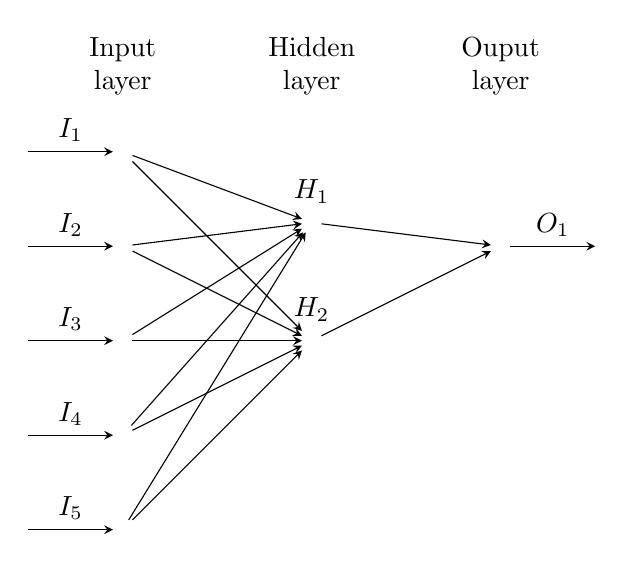
\begin{tikzpicture}[x=1.2cm, y=1.2cm, >=stealth]

\foreach \m/\l [count=\y] in {1,2,3,4,5}
  \node [every neuron/.try, neuron \m/.try] (input-\m) at (0,2.5-\y) {};

\foreach \m [count=\y] in {1, 2}
  \node [every neuron/.try, neuron \m/.try ] (hidden-\m) at (2,2-\y*1.25) {};

\foreach \m [count=\y] in {1}
  \node [every neuron/.try, neuron \m/.try ] (output-\m) at (4,1.5-\y) {};

\foreach \l [count=\i] in {1,2,3,4,5}
  \draw [<-] (input-\i) -- ++(-1,0)
    node [above, midway] {$I_\l$};

\foreach \l [count=\i] in {1,2}
  \node [above] at (hidden-\i.north) {$H_\l$};

\foreach \l [count=\i] in {1}
  \draw [->] (output-\i) -- ++(1,0)
    node [above, midway] {$O_\l$};

\foreach \i in {1,...,5}
  \foreach \j in {1,...,2}
    \draw [->] (input-\i) -- (hidden-\j);

\foreach \i in {1,...,2}
  \foreach \j in {1}
    \draw [->] (hidden-\i) -- (output-\j);

\foreach \l [count=\x from 0] in {Input, Hidden, Ouput}
  \node [align=center, above] at (\x*2,2) {\l \\ layer};
\end{tikzpicture}
\caption{Example ANN Architecture}
\end{figure}

\begin{figure}
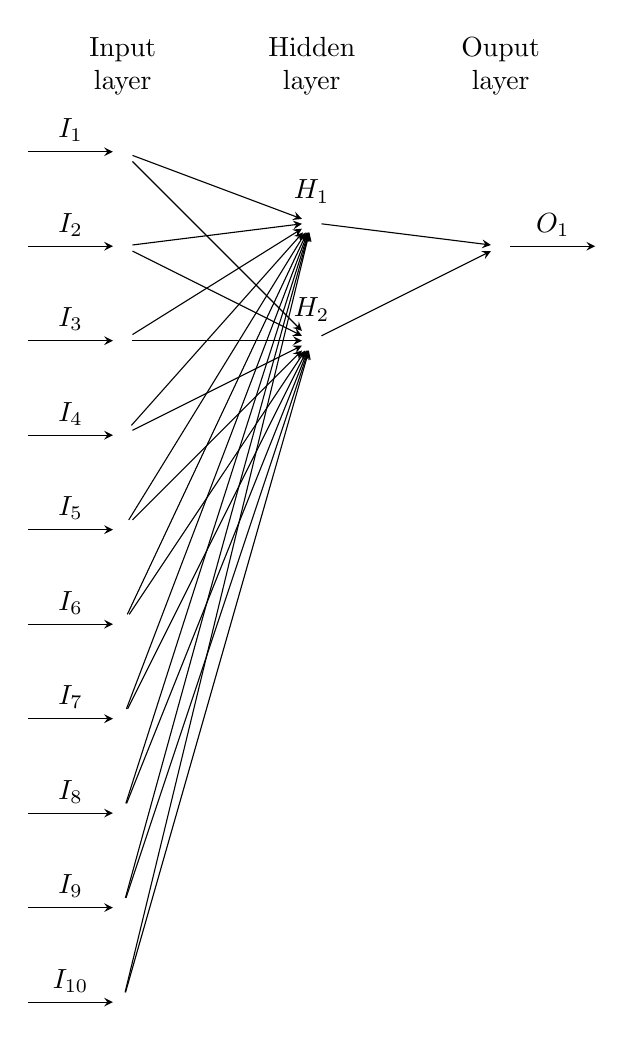
\begin{tikzpicture}[x=1.2cm, y=1.2cm, >=stealth]

\foreach \m/\l [count=\y] in {1,2,3,4,5,6,7,8,9,10}
  \node [every neuron/.try, neuron \m/.try] (input-\m) at (0,2.5-\y) {};

\foreach \m [count=\y] in {1, 2}
  \node [every neuron/.try, neuron \m/.try ] (hidden-\m) at (2,2-\y*1.25) {};

\foreach \m [count=\y] in {1}
  \node [every neuron/.try, neuron \m/.try ] (output-\m) at (4,1.5-\y) {};

\foreach \l [count=\i] in {1,2,3,4,5,6,7,8,9,10}
  \draw [<-] (input-\i) -- ++(-1,0)
    node [above, midway] {$I_{\l}$};

\foreach \l [count=\i] in {1,2}
  \node [above] at (hidden-\i.north) {$H_\l$};

\foreach \l [count=\i] in {1}
  \draw [->] (output-\i) -- ++(1,0)
    node [above, midway] {$O_\l$};

\foreach \i in {1,...,10}
  \foreach \j in {1,...,2}
    \draw [->] (input-\i) -- (hidden-\j);

\foreach \i in {1,...,2}
  \foreach \j in {1}
    \draw [->] (hidden-\i) -- (output-\j);

\foreach \l [count=\x from 0] in {Input, Hidden, Ouput}
  \node [align=center, above] at (\x*2,2) {\l \\ layer};
\end{tikzpicture}
\caption{ANN Architecture for Epworth Sleepiness Scale}
\end{figure}

\begin{figure*}[h]
    \centering
    \includegraphics[width=1.9\columnwidth]{models/epworth tree.png}
    \caption{Epworth Sleepiness Scale Decision Tree Model}
    \label{fig:epworthTree}
\end{figure*}
\begin{figure*}[h]
    \centering
    \includegraphics[width=1.9\columnwidth]{models/sleep disturbance tree.png}
    \caption{Sleep Disturbance Decision Tree Model}
    \label{fig:disturbanceTree}
\end{figure*}
\begin{figure*}[h]
    \centering
    \includegraphics[width=1.9\columnwidth]{models/zung tree.png}
    \caption{Zung Depression Scale Decision Tree Model}
    \label{fig:zungTree}
\end{figure*}



%%{\color{red} The trees looks very tiny %and fuzzy. Please try to enhance the %figures}
%\label{Decision Trees}
%\begin{figure*}[h]
    %\centering
    %\includegraphics[width=1.9\columnwidth]{sleep habits tree.png}
    %\caption{Sleep Habits Questionnaire Decision Tree}
    %\label{fig:sleepHabitsTree}
%\end{figure*}
%\begin{figure*}[h]
    %\centering
    %\includegraphics[width=1.9\columnwidth]{models/epworth tree.png}
    %\caption{Epworth Sleepiness Scale Questionnaire Decision Tree}
    %\label{fig:epworthTree}
%\end{figure*}
%\begin{figure*}[h]
    %\centering
    %\includegraphics[width=1.9\columnwidth]{models/sleep disordered breathing tree.png}
    %\caption{Sleep Disordered Breathing Questionnaire Decision Tree}
    %\label{fig:breathingdisTree}
%\end{figure*}
%\begin{figure*}[h]
    %\centering
    %\includegraphics[width=1.9\columnwidth]{models/sleep disturbance tree2.png}
    %\caption{Sleep Disturbance Questionnaire Decision Tree}
    %\label{fig:disturbanceTree}
%\end{figure*}
%\begin{figure*}[h]
    %\centering
    %\includegraphics[width=1.9\columnwidth]{models/zungsimptree3.png}
    %\caption{Simplified Zung Depression Scale Questionnaire Decision Tree}
    %\label{fig:zung}
%\end{figure*}
%
%\label{Neural Networks}
%\begin{figure}[h]
    %\centering
    %\includegraphics[width=0.9\columnwidth]{models/Models 4-20/Sleep Habits.jpg}
    %\caption{Sleep Habits Questionnaire Neural Network}
    %\label{fig:sleepHabitsNN}
%\end{figure}
%\begin{figure}[h]
    %\centering
    %\includegraphics[width=0.9\columnwidth]{models/Models 4-20/Zung Neural Network.jpg}
    %\caption{Zung Depression Scale  Questionnaire Neural Network}
    %\label{fig:zungNeural}
%\end{figure}
%\begin{figure}[h]
    %\centering
    %\includegraphics[width=0.9\columnwidth]{models/Models 4-20/Zung Neural Network Modified.jpg}
    %\caption{Simplified Zung Depression Scale  Questionnaire Neural Network}
    %\label{fig:zungNeuralSimp}
%\end{figure}
%\begin{figure}[h]
    %\centering
    %\includegraphics[width=0.9\columnwidth]{models/Models 4-20/Epworth.jpg}
    %\caption{Epworth Sleepiness Scale  Questionnaire Neural Network}
    %\label{fig:epworthNeural}
%\end{figure}
%\begin{figure}[h]
    %\centering
    %\includegraphics[width=0.9\columnwidth]{models/Models 4-20/Sleep Disordered Breathing.jpg}
    %\caption{Sleep Disordered Breathing  Questionnaire Neural Network}
    %\label{fig:disdorderedNeural}
%\end{figure}
%\begin{figure}[h]
    %\centering
    %\includegraphics[width=0.9\columnwidth]{models/Models 4-20/Sleep Disturbance.jpg}
    %\caption{Sleep Disturbance Questionnaire Neural Network}
    %\label{fig:disturbanceNeural}
%\end{figure}



\subsection{Analysis}

When examining the accuracy of these models, it can be seen that they all possess similar rates of correct classifications. With a standard deviation of 0.074 the differences between the models is negligible. The models with the highest accuracy is the Zung Depression Scale neural network model with an accuracy of 0.871 and the Zung Depression Scale decision tree model with an accuracy of 0.871. The Zung Depression Scale models also boast the highest values for precision and sensitivity, those metrics also boast low standard deviations of 0.067 and 0.075 respectively. Due to the low standard deviation, the performance of the models in relation to those metrics are all similar. \par
When examining the MCC values for the models, the lowest value is the Epworth Sleepiness Scale MCC with a value of 0.415 and the highest value is the Zung Depression Scale neural network with an MCC of 0.743. The MCC provides a quick metric by which to measure the general effectiveness of the models. With values ranging from roughly 0.4 to 0.75, the models can be judged as performing well with results that skew towards making correctly classifications the majority of the time. The closer the MCC is to zero the more random its classification is, with an MCC value of 0.743 for its neural network model and an MCC value of 0.727 for its decision tree model the performance of the Zung Depression Scale models are the closest to always correct classification. \par
The effectiveness of each model is also judged by their confusion matrix values. In medical testing the amount of false negatives is an important metric. In these models a false negative reflects the model predicting that no sleep apnea is present in the patient when there is sleep apnea present. The models all show false negative counts in the range of 41 to 87 with a standard deviation of 16.488. The Epworth Sleepiness Scale decision tree model possesses the highest amount of false negatives with a count of 87(\autoref{epworthDecisionMatrix}). This is a rate of 11\% of the classifications resulting in a false negative. The models with the lowest amount of false negatives are the Zung Depression Scale models with a count of 48 for its decision tree models(\autoref{zungDecisionMatrix}) and a count of 41 for its neural network model(\autoref{zungNeuralMatrix}). Despite the higher rate of false negatives in its decision tree model, the Epworth Sleepiness Scale neural network has a low count of false negatives with a total of 54 (\autoref{epworthNeuralMatrix}). \par
The amount of false positives in these models ranges from 61 to 185 with a standard deviation of 55.825. A false positives represents when the model predicts the presence of sleep apnea when there is no sleep apnea present. While this is not as significant in medical testing as false negatives, a false positive will result in further testing when none is needed and will nullify the goal of these models in reducing the amount of unneeded testing. The Epworth Sleepiness Scale neural network model has the highest amount of false negatives with 185 (\autoref{epworthNeuralMatrix}), this is 23\% of the full data set that was tested for this model. The Sleep Disturbance questionnaire also possesses high false negative models with a count of 164 (\autoref{disturbDecisionMatrix}) for its decision tree model and a count of 154 (\autoref{distrubNeuralMatrix}) for its neural network model. The Zung Depression Scale boasts the lowest count of false positives in its model, possessing a total of 61 false positives in its decision tree model (\autoref{zungDecisionMatrix}) and 62 in its neural network model (\autoref{zungNeuralMatrix}).\par


\begin{table*}[ht]
\centering
\begin{tabular}{@{}lllllllllll@{}}
\toprule
                                    & Correctly Classified (\%) & TP     & FN     & FP     & TN     & Precision & Sensitivity & Accuracy & F-Measure & MCC   \\ \midrule
\textbf{Zung Depression Scale}      &                           &        &        &        &        &           &             &          &           &       \\
\rowcolor[HTML]{EFEFEF} 
j48                                 & 86.358                    & 331    & 48     & 61     & 359    & 0.864     & 0.864       & 0.864    & 0.864     & 0.727 \\
\rowcolor[HTML]{EFEFEF} 
MultilayerPerceptron                & 87.109                    & 330    & 41     & 62     & 366    & 0.872     & 0.871       & 0.871    & 0.871     & 0.743 \\
\textbf{Epworth Sleepiness Scale}   &                           &        &        &        &        &           &             &          &           &       \\
\rowcolor[HTML]{EFEFEF} 
j48                                 & 78.875                    & 298    & 87     & 82     & 333    & 0.789     & 0.789       & 0.789    & 0.789     & 0.577 \\
\rowcolor[HTML]{EFEFEF} 
MultilayerPerceptron                & 70.125                    & 195    & 54     & 185    & 366    & 0.721     & 0.701       & 0.701    & 0.690     & 0.415 \\
\textbf{Sleep Disturbance}          &                           &        &        &        &        &           &             &          &           &       \\
\rowcolor[HTML]{EFEFEF} 
j48                                 & 72.716                    & 231    & 54     & 164    & 350    & 0.745     & 0.727       & 0.727    & 0.721     & 0.471 \\
\rowcolor[HTML]{EFEFEF} 
MultilayerPerceptron                & 72.215                    & 241    & 68     & 154    & 336    & 0.732     & 0.722       & 0.722    & 0.719     & 0.454 \\
%\textbf{Standard Deviation(sample)} & 7.442                     & 56.720 & 16.488 & 55.825 & 14.569 & 0.067     & 0.075       & 0.074    & 0.078     & 0.143 \\ 
\bottomrule
\end{tabular}
\caption{Model Testing Results and Calculations}
\label{tab:results}
\end{table*}



\subsection{Conclusions}

Through looking at the various metrics provided, it can be concluded that the Zung Depression Scale models shows the highest performance. With the lowest count of false negatives and a high rate of accuracy as well as a high MCC value, the models perform well in relation to the metrics important in medical diagnoses. The Zung Depression Scale questionnaire focuses on the self-rated severity of depression symptoms that the subjects feel. As discussed earlier, sleep disordered breathing is often linked to various mental disorders such as depression\cite{clevelandClinic}. The effectiveness of the models trained on this questionnaire further shows the strong correlation between the two disorders. The Zung Depression Scale questionnaire also possess the highest number of variables between all the questionnaires. It created the most expansive decision tree model (\autoref{fig:zungTree}) and neural network (\autoref{zungNeuralInputs}) of the questionnaires as a result of this. This abundance of variables present in this questionnaire may also be contributing to the higher rate of success it boasts. \par
Despite the high performance of the Zung Depression Scale models, the other models also possess high accuracy, sensitivity and precision ratings and are successful in diagnosing sleep apnea and suggesting further testing relatively reliably. The MCC of each model being roughly 0.5 shows that their classifications are by no means random though the effectiveness of each does vary as seen in the confusion matrix of each model. With low standard deviations across the board for all metrics, each model can be judged as being effective.


\subsection{Limitations}

An important aspect to consider in this study is the relatively low number of positive sleep apnea patients in the study. As seen in \autoref{tab:apneaCounts}, the number of positive sleep apnea diagnoses present in the data set is roughly 18\% of the total data points. This skewed proportion is why each questionnaire was parsed down and relation tuples were deleted in order to bring the count of positive and apnea classifications to a more even amount. The apnea counts for this smaller table can be seen in \autoref{smallApneaCounts}. If there were a higher amount of positive apnea classifications present in the data set and it could be expaned with more data, the models would most likely have an increased effectiveness.\par




Another factor in this data set is the variable number of visits and tests that each subject underwent. Each subject had between one to four visits each, and each time would fill out all questionnaires. Though their questionnaire answers may change, their sleep apnea diagnosis would not. These multiple visits may have skewed the data as well. \par
The final limitation is the size of the Zung Depression Score questionnaire. With a total of 22 variables in the data set, the models built for the data set are all complex and the visual representations of the models are messy and difficult to read. In an attempt to simplify the models, a simplified Zung Depression Scale model was tested by utilizing Wekas built-in filters and deleting various amounts of variables that affect the model the least. This resulted in a model with less variables and more organized models. However, the simplified model had significantly worse performance than the full model and was abandoned as a result of those poor results.


\section{Acknowledgements}
This Wisconsin Sleep Cohort Study was supported by the U.S. National Institutes of Health, National Heart, Lung, and Blood Institute (R01HL62252), National Institute on Aging (R01AG036838, R01AG058680), and the National Center for Research Resources (1UL1RR025011). The National Sleep Research Resource was supported by the U.S. National Institutes of Health, National Heart Lung and Blood Institute (R24 HL114473, 75N92019R002). \cite{Young2009}\cite{Zhang2018}





%============================================
\bibliographystyle{IEEEtran}
\bibliography{refs}
%============================================
\end{document}